\input{doctools/latex/notes_template.tex} % Page setup
\input{doctools/latex/mycommands.tex} % Some useful commands

\newlength{\pad} \setlength{\pad}{.2cm}

\begin{document}
% \doublespacing %set double spacing


% Title
\thispagestyle{empty} %First page does not need headers and footers
\begin{center}
  {\huge gEDA notes}\\
  \today
\end{center}
\clearpage

% Table of contents
\pagestyle{toc}
\tableofcontents
\clearpage \pagestyle{normal}


\part{Working with projects in general}

% The GEDA configuration files
\section{gEDA configuration files}

\subsection{The \texttt{gafrc} file}
The gEDA suite consists of many different tools, which often need to know where your component libraries are.  The \texttt{gafrc} file is a repository for this information.  I like to keep this file in the schematics directory of an individual project.  This way I can limit how my projects affect each other.  

Here's an excerpt from pencils project's \texttt{gafrc} file:

\filesnip{~/projects/pencils/implement/schematics/gafrc}{
\verbatiminput{gafrc_sample.txt}
}

The individual tools can be further customized with individual \texttt{rc} files like \texttt{gschemrc}, which are then also placed in the \verb8~./gEDA8 directory.

\subsection{The \texttt{gschemrc} file}
The configuration options available for your local \verb8~./gEDA/gschemrc8 are shown in the ``system-gschemrc'' file.  On my machine, this file is located in
\begin{center}
\begin{minipage}{5cm}
\verb8/usr/share/gEDA/system-gschemrc8.
\end{minipage}
\end{center}


\subsection{PCB configuration}
The configuration file for PCB will vary with the GUI toolkit PCB was compiled with.  Both lesstif and gtk are supported as of \verb8pcb-200604148.  Use
\begin{center}
\begin{minipage}{2cm}
\verb8pcb -h8
\end{minipage}
\end{center}
and look for ``Available GUI hid:'' to determine what's been installed and see a list of configuration options.  The double-dash options correspond to X and gtk resources.  Example:
\begin{center}
\begin{minipage}{7cm}
Command line:\\
\verb8pcb --grid-color '#ff0000'8\\

.Xdefaults (for lesstif toolkit):\\
\verb8pcb.grid-color: #ff00008\\

\$HOME/.pcb/preferences (for gtk toolkit):\\
\verb8grid-color = #ff00008
\end{minipage}
\end{center}

%You can also print and export right from the command line.  We use
%this to generate the documentation; the "master" for illustrations are
%.pcb files!  We invoke pcb from the Makefile to build png (for html),
%eps (for dvi), and pdf (for pdf) formats for each board for inclusion
%in the documentation.


% File maitenence etiquette
\section{Project file etiquette}
For consistency:
\begin{itemize}
    \item A project usually consists of more than one schematic file.  The collection of files should be put under version control, so that the filenames themselves never pick up a version number.
    \item \verb8gsch2pcb8 will tack ``.pcb'' on to the string you give it as ``output-name,'' so you don't need to add it.  The generated file should be moved to the layout directory.  There it should be versioned to keep track of changes.  The netlist should not be versioned since it is generated by the schematic.
    \item If a schematic has more than one page, the first page should be a table of contents.
    \item If the ECO changes the BOM, modify it by hand and append \verb8_eco8 to the filename. I won't bother keeping track of multiple rounds of ECOs -- each new ECO should just overwrite the \verb8_eco8 BOM.  If there's a website with the BOM on it, the BOM should be updated to the \verb8_eco8 version.
\end{itemize}

\clearpage
\subsection{Directory structure}
\label{project_structure_subsection}
A nice directory structure looks like this:
\begin{itemize}
    \item \textbf{project} -- The top-level directory.
        \begin{itemize}
            \item \textbf{datasheets} -- Datasheets for parts used in the project.
            \item \textbf{eda} -- Version-controlled eda tools.
                \subitem Check out using \texttt{svn checkout svn://www.jrranalytics.com/eda}
            \item \textbf{proto} -- Version-controlled prototyping tools.
                \subitem Check out using \texttt{svn checkout svn://www.jrranalytics.com/proto}
            \item \textbf{notes} -- Design notes for the project.
                \subitem \textbf{doctools} -- Version-controlled documentation tools.
                    \subsubitem Check out using \texttt{svn checkout svn://www.jrranalytics.com/doctools}
            \item progress.org -- Progress notes to be edited with org-mode.
            \item \textbf{reva} -- Letter-coded revision directory.
                \begin{itemize}
                    \item \textbf{data}
                    \item \textbf{drawings} -- Mechanical drawings for the revision.
                    \item \textbf{schematics} -- Electrical schematic pages
                        \subitem \textbf{kit2} -- Number-coded directory generated with the \textit{kitgen} script.
                    \item \textbf{layout} -- Circuit board layout
                    \item \textbf{pictures}
                \end{itemize}
        \end{itemize}
\end{itemize}

\subsection{Preparing a project for version control}

\boxcmd{\$ mkdir project \\
        \$ mkdir project/datasheets \\
        \$ mkdir project/notes \\
        \$ touch project/progress.org \\
        \$ mkdir project/reva \\
        \$ mkdir project/reva/data \\
        \$ mkdir project/reva/drawings \\
        \$ mkdir project/reva/schematics \\
        \$ mkdir project/reva/layout \\
        \$ mkdir project/reva/pictures \\
        \$ mkdir project/reva/howto \\
        \$ mkdir project/reva/code \\
        \$ svn import ./project svn://www.jrranalytics.com/projects/project -m "Initial import" \\
        \$ mv project project\_nosvn \\
        \$ svn checkout svn://www.jrranalytics.com/projects/project \\
        \$ rm -rf project\_nosvn
}
Now add the subversion externals:
\boxcmd{\$ cd project \\
        \$ svn propedit svn:externals .
}
...which will prompt you to edit a file defining the externals.  Add the lines
\filesnip{svn-prop.tmp}{eda svn://www.jrranalytics.com/eda \\
            eda/notes/geda/doctools svn://www.jrranalytics.com/doctools \\
            eda/notes/avr/doctools svn://www.jrranalytics.com/doctools \\
            notes/doctools svn://www.jrranalytics.com/doctools \\
            reva/howto/doctools svn://www.jrranalytics.com/doctools
}
to any other externals you'd like to define.  Now a simple \texttt{svn update} will bring in the externals.

\rednote{You must create a task tagged with the project name after creating a project.  The top-level task name should be ``\texttt{* TODO Work on} \textit{project name}'', with a link to the project location below as a comment.}

\subsection{Using the \texttt{makeproj.py} script}
The \texttt{makeproj.py} script automates project creation by creating the directories detailed in section \ref{project_structure_subsection}.  To use it, first edit end script to customize your project's name, home directory, and revision letter.  Then the command
\boxcmd{\$ python makeproj.py}
will create the project.

The script can also make a new revision of an existing project.  Just change the revcode while leaving the existing project name and directory.


\part{Capture with gschem}

% Making symbols for capture
\section{Making symbols for gschem}
Using \texttt{gschem} itself is one way to view and modify device attributes.  This section will describe how to use \texttt{gschem} to create and modify parts to be used in schematics. 

\rednote{When you include a part in a schematic, \texttt{gschem} associates the part filename with the schematic.  Thus, changes made to the part files outside of the schematic will automatically update to the schematic.  This is bad when you ``translate'' the symbol when editing it, because the symbol will then move around on all the schematics it's associated with.}

\subsection{Making symbols for electrical and non-electrical parts}
Electrical symbols are those that have pins and make connections you can describe with a netlist.  Non-electrical symbols are for parts like nuts and bolts that should be included in the bill of materials but not the netlist.  Non-electrical parts need the \texttt{device}, \texttt{part}, \texttt{refdes}, and \texttt{value} attributes.

\subsubsection{Making a new symbol from scratch}

%Numbered directions for making gschem part
\begin{enumerate}
\item Run \texttt{gschem} -- bring up a blank schematic page.  Get rid of the default titleblock.
\item Draw the symbol
    \subitem Lines and pins should be drawn with 0.1 inch snap to grid.  Use  \textsl{Options} $\rightarrow$ \textsl{Snap grid spacing} to set grid size and be sure to turn snapping on.

\item (Electrical symbols) Add pins with \textsl{Add} $\rightarrow$ \textsl{pin}
    \subitem Pins should be 0.3 inches long and have their red ends pointing away from the symbol -- net connections are made at the red ends
    \subitem Pins should be at least 0.4 inches from their neighbors

\item (Electrical symbols) Add pin attributes: \texttt{pinnumber}, \texttt{pinseq}, \texttt{pinlabel}
    \subitem \texttt{pinseq} just tells gschem the order to output pins when it makes a netlist.
    \subitem The \texttt{pinnumber} attribute must match up with the ones you use for your footprints.  This will label pins on the netlist, so make this ``value only'' visible.  If you want the pin number to be visible, it should be positioned 50 mils away from its pin.
    \subitem The \texttt{pinlabel} attribute is just for information.  It lets you find the pin entry if you ever need to edit the raw text file for the symbol.


\item (Electrical symbols) Add the component's footprint attribute
    \subitem Make this attribute invisible, but edit the attribute (after turning the invisible text on) to select ``show name and value.''  Then both the attribute name and value will show up when you display invisible text.
    \subitem Example: \verb8footprint=2pin_MTA100_pol8
    
    \nailnote{Look in the project's eda\textbackslash footprints for available footprints.  The file footnotes.org may have some footprint-specific notes.  Use \texttt{\$pcb footprint.fp} to see a footprint.  See section \ref{footprint_section} beginning on page \pageref{footprint_section} for more information about footprints.}

\item Add the component's device attribute
    \subitem The device attribute is required for using \texttt{gnetlist} later on
    \subitem The device attribute is the basic part description, like \texttt{resistor}, \texttt{capacitor}, or \texttt{opamp}
    \subitem This should be made invisible

    
\item Add the component's ``value'' attribute
    \subitem This is the flavor of the device.  This will appear on the schematic to label the symbol along with the reference designator, so make this ``value only'' visible.  Feel free to insert spaces or symbols in this field, since it's only for the user's information.
        \subsubitem Resistors -- the resistor value
        \subsubitem Opamps -- the basic part number without package or other suffixes
        \subsubitem Zeners -- the basic part number.  The zener voltage can go in the optional ``label'' attribute
        \subsubitem Connectors -- a description of the connector, like ``polarized MTA100''
        \subsubitem Screws -- The pitch and length, like 6-32 x 5/16 phillips.

\item Add the Faulhaber Labs part number in a ``part'' field.  These fields can just be typed in -- they don't have to be members of the pull-down list.  This part field will reference another database containing purchasing information and other comments.
    \subitem Example: \texttt{part=14-6}    

    
\item (optional) Add a \texttt{label} attribute for things like zener voltages or resistor power ratings.  The \texttt{label} attribute also isn't in the default pull-down list -- you have to write it in.  Make this value visible.  Just writing things like this in text prohibits them from rotating relative to the symbol.
    
\item Add a reference designator (\texttt{refdes})
    \subitem Adding a designator like U? allows gschem to choose a value for ? when the device is in a schematic.
    
\item Translate the symbol to the origin
    \subitem \textsl{Edit} $\rightarrow$ \textsl{Symbol translate}
    \subitem Keep all the invisible text visible when translating.  Otherwise it will be translated out of the window.

\item Save your component with the filename \texttt{partname.sym}.  The save dialog box allows you to choose whether you save things as a schematic or a symbol, but it does the same thing regardless of your selection.
\end{enumerate}

%To make these symbol figures, screen grab the gschem window with xv and save to png (full color).  Open the png with gthumb and apply the negative, desaturate, and equalize transformations.  Save as png again.  Open again with gimp and save as postscript

Figures \ref{nice_opamp}, \ref{nice_resistor}, and \ref{non_electric} show examples of what you should see when you're done with a symbol.

\begin{figure}[ht]
    \begin{center}
        \includegraphics[clip,scale=0.3]{opa134-a.ps}
        \caption{A nice-looking opamp symbol with all invisible attributes showing.  This opamp has a separate power symbol that doesn't need any symbol attributes, only pin attributes.\label{nice_opamp}}
    \end{center} 
\end{figure}

\begin{figure}[ht]
    \begin{center}
        \includegraphics[clip,scale=0.3]{100_1206.ps}
        \caption{A nice-looking resistor with all invisible attributes showing\label{nice_resistor}}
    \end{center} 
\end{figure}

\begin{figure}[ht]
    \begin{center}
        \includegraphics[clip,scale=0.4]{wall_xformer_24v_1a.ps}
        \caption{A non-electrical component\label{non_electric}}
    \end{center} 
\end{figure}


\clearpage
\subsubsection{Making multi-part symbols}
Multi-part symbols are those for which two or more symbols are used to represent a single part.  Making them amounts to simply making multiple symbols and naming their files suggestively.  For example, two symbols describing a \mfgpart{opa134} op amp could be named \urlname{opa134a} and \urlname{opa134b}.  You'll have to remember that these two files are related.  

The way \progname{gnetlist} handles multi-part symbols seems to be a work in progress.  These rules seem to hold for \progname{geda} version 1.6.2:
\begin{enumerate}
    \item All symbols representing the same part must share the same reference designator.  For example, the \urlname{opa134a} and \urlname{opa134b} symbols could both have the \texttt{U1} reference designator, but not \texttt{U1a} and \texttt{U1b}.
    \item Only the ``first'' part of a muti-part symbol should have anything other than the reference designator defined.  Attributes like the footprint name or the part number will be ignored for parts placed after the first part.
\end{enumerate}

\rednote{\progname{gschem} adds entries to a schematic file as they are added with the graphical editor.  Symbols placed chronologically before others will appear at lower line numbers.  The netlister scans the schematic file from top to bottom.  If it finds two symbols with the same reference designator, it will use attributes from the first one and ignore those from the second.} 



\clearpage
\subsection{Making power, ground, and other net symbols}
%net symbols
Net symbols consist of a graphic, a pin, and a net attribute.  To edit the net attribute at the schematic level,  add the attribute as an overall symbol attribute as shown in Fig.\ \ref{symbol_net} -- not one associated with the symbol's pin.   Since these net symbols only have one pin, this attribute always looks something like \texttt{name:1}.  After placing the symbol on the schematic, change the name of the net attribute as needed.  The name should then look like \texttt{+9V:1} or \texttt{input:1} etc.  

There doesn't seem to be a way to avoid including the pin number with the name if you want to be able to change the net name on the schematic.  Another way to make these symbols is to permanently associate a net name with the symbol, and then just add a text label like \texttt{+9V} to the symbol.  This scheme is illustrated in Fig.\ \ref{symbol_nonet}.  You would have to have a different symbol file for each net you want to have a symbol for.
%To make these symbol figures, screen grab the gschem window with xv and save to png (full color).  Open the png with gthumb and apply the negative, desaturate, and equalize transformations.  Save as png again.  Open again with gimp and save as encapsulated postscript.
\begin{figure}[ht]
	\begin{center}
		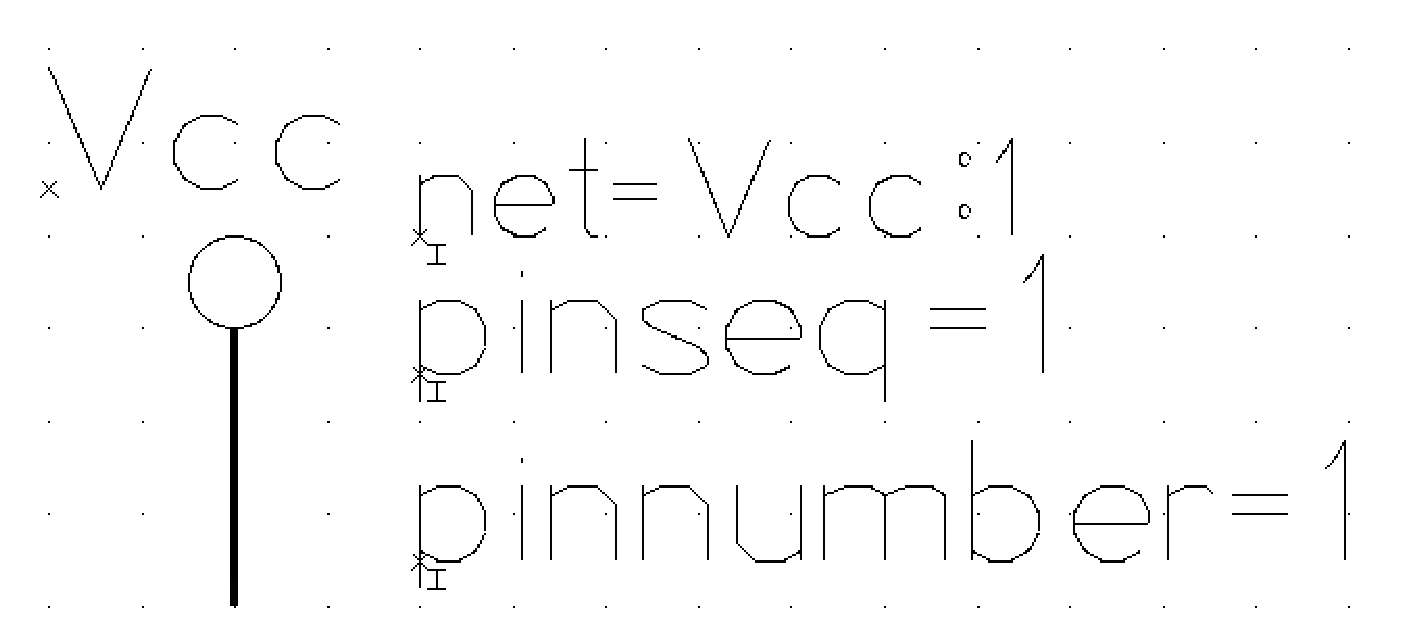
\includegraphics[clip,scale=0.2]{generic_vcc.eps}
		\caption{A power symbol with a hard-wired net attribute.  The attributes to the right of the symbol are made invisible on the schematic.\label{symbol_nonet}}
	\end{center} 
\end{figure}

\begin{figure}[ht]
	\begin{center}
		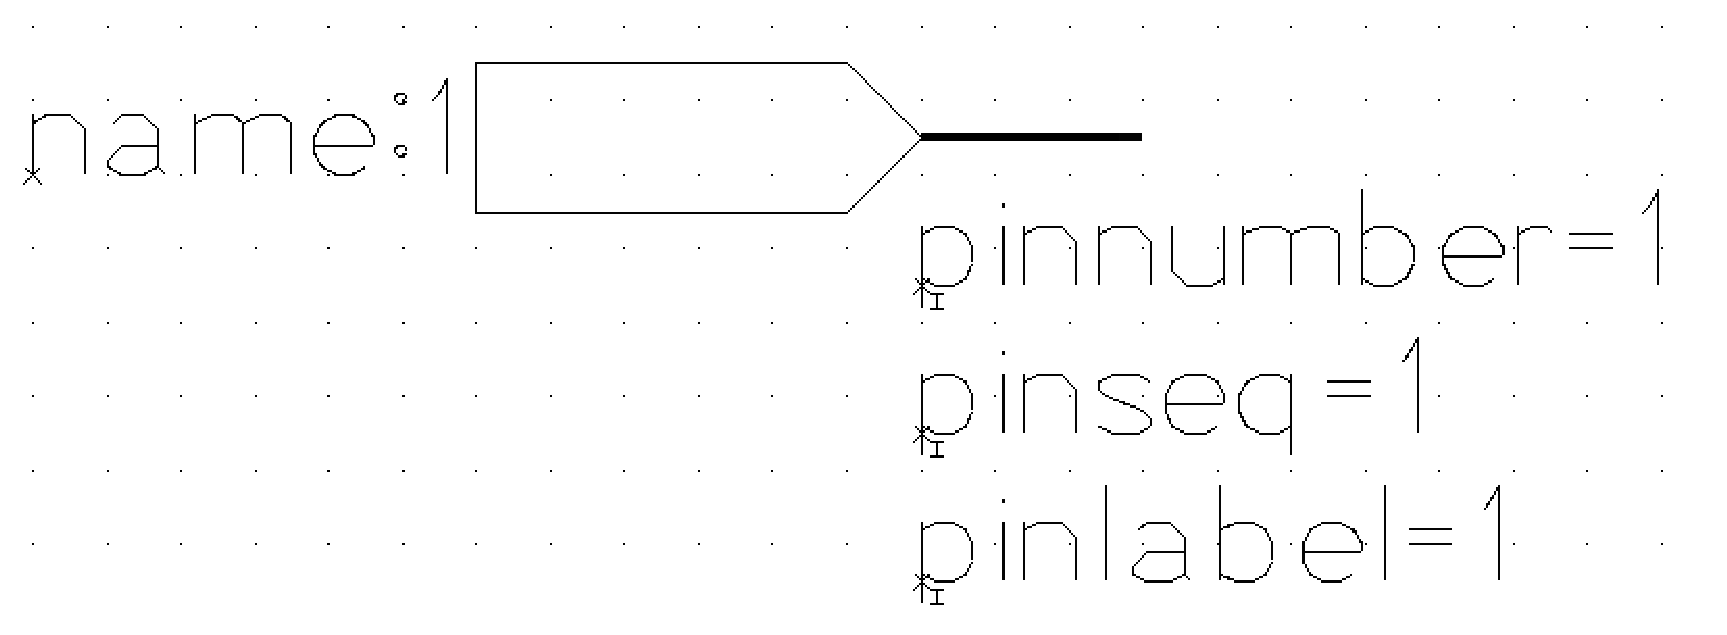
\includegraphics[clip,scale=0.2]{input_netname.eps}
		\caption{An off-page connector symbol with a net attribute you can change at the schematic level.  The attributes to the right of the symbol are made invisible on the schematic.\label{symbol_net}}
	\end{center} 
\end{figure}


\clearpage
\subsection{Changing attributes at the schematic level}
A part's default attributes can be overridden by editing the part within your schematic.  Selecting the part and clicking \textsl{Edit} $\rightarrow$ \textsl{Edit} (or using the \texttt{ee} shortcut) will bring up an ``Edit Attributes'' dialog box.  Here you can add new attributes to override the defaults.  For example, adding an attribute with the name ``footprint'' will override the footprint attribute taken from the symbol file.

%Miscellaneous notes
\subsection{General notes}
\begin{itemize}
    \item When you start gschem on a blank page, you'll be zoomed way out.  Zoom in a lot until the lines you draw snap to your visible grid.
    \item Multi-part devices should have a separate symbol for each part, named like part-a, part-b, etc.  For example, a single op-amp should have two symbols: one for the amplifier and one for its power pins.  Only the first device needs to have all the attributes -- the following devices only need reference designators.
    \item Op-amp symbols should be 0.8 inches high by 0.6 inches long.
    \item If a new device has the same symbol as one you've already drawn, just edit the text file and save it as a new part.
    \item Canned symbols are in \texttt{/usr/share/gEDA/sym}
    \item No line feeds are allowed in symbol files
    \item Part attributes must be associated with text -- you can't have a name=attribute entry in a symbol file without also having a text formatting line immediately above it.  This means that the pinnumber, pinseq, and pinlabel attributes will pile up on the schematic page if you make them visible.
\end{itemize}






\section{Working with \texttt{gschem}}


%%%%%%%%%%%%%%%%%%%%%%%%%%%%%%%%%%%%%%%%%%%%%%%%%%%%%%%%%%%%%%%%%%%%%%%%%%%
%Keyboard shortcuts
%%%%%%%%%%%%%%%%%%%%%%%%%%%%%%%%%%%%%%%%%%%%%%%%%%%%%%%%%%%%%%%%%%%%%%%%%%%
\subsection{Keyboard shortcuts}
Some keyboard shortcuts are shown in table \ref{shortcuts}.  A comprehensive list is brought up with \textsl{Help} $\rightarrow$ \textsl{Hotkeys} or with the \texttt{hh} key sequence.

\begin{table}[h]
	\begin{center}
	\setlength{\extrarowheight}{0.5cm}
		\begin{tabular}{cl}
		Key sequence	&Function\\
		\hline
		z		&Zoom in\\
		Shift + z	&Zoom out\\
		en		&Show/hide invisible text\\
		l		&Start drawing a line (like for a symbol)\\
		s		&Exit whatever mode you're in and go back to select mode\\
		m		&Begin moving a selected object\\
		ex		&Bring up the single attribute editor within a schematic\\
		\end{tabular}
		\caption{gschem keyboard shortcuts \label{shortcuts}}
	\end{center}
\end{table}

%%%%%%%%%%%%%%%%%%%%%%%%%%%%%%%%%%%%%%%%%%%%%%%%%%%%%%%%%%%%%%%%%%%%%%%%%%%
%Adding text to schematics
%%%%%%%%%%%%%%%%%%%%%%%%%%%%%%%%%%%%%%%%%%%%%%%%%%%%%%%%%%%%%%%%%%%%%%%%%%%
\subsection{Adding text}
The key combination \texttt{a}$\rightarrow$\texttt{t} brings up a text entry box.  Entered text can be edited using the \texttt{e}$\rightarrow$\texttt{x} sequence.  Nice-looking text sizes are shown in table \ref{text_sizes}.

\begin{table}[ht]
	\begin{center}
		\begin{tabular}{|c|c|}
		\hline
		\textbf{Text}	&\textbf{Size}\\
		\hline \hline
		Comments	&12\\
		\hline
		Headings, like ``notes'' or ``changes on this page''	&18\\
		\hline
		\end{tabular}
		\caption{Text sizes for notes on schematic pages\label{text_sizes}}
	\end{center}
\end{table}


%%%%%%%%%%%%%%%%%%%%%%%%%%%%%%%%%%%%%%%%%%%%%%%%%%%%%%%%%%%%%%%%%%%%%%%%%%%
%Making pretty prints
%%%%%%%%%%%%%%%%%%%%%%%%%%%%%%%%%%%%%%%%%%%%%%%%%%%%%%%%%%%%%%%%%%%%%%%%%%%
\subsection{Making pretty prints}
You can print to postscript with \textsl{File} $\rightarrow$ \textsl{Print} and then choosing a filename.  You can print from the command line using
\boxcmd{\$ gschem -s /usr/share/gEDA/scheme/print.scm -o output.ps -p input.sch}
where \texttt{input.sch} is the schematic to be printed to \texttt{output.ps}. 

\subsubsection{Fixing text alignment}
Pieces of text have alignment marks associated with them.  When the text is printed, these marks will stay put as the text grows or shrinks to accomodate whatever fonts are used by the output device.  You'll thus want to align the alignment marks if you want text objects to line up in your print.  There are two tricks to this:



\begin{enumerate}
	\item Rotate the text until the alignment mark is where you want it.  Notice that \texttt{gschem} refuses to write text upside down.
	\item Use the \texttt{ex} sequence to edit the alignment mark position of a text attribute associated with a symbol.
\end{enumerate}



%%%%%%%%%%%%%%%%%%%%%%%%%%%%%%%%%%%%%%%%%%%%%%%%%%%%%%%%%%%%%%%%%%%%%%%%%%%
%Miscellaneous notes
%%%%%%%%%%%%%%%%%%%%%%%%%%%%%%%%%%%%%%%%%%%%%%%%%%%%%%%%%%%%%%%%%%%%%%%%%%%
\subsection{Miscellaneous notes}

\begin{itemize}
	\item 
\end{itemize}



% Working with gnetlist
%netlist
\section{Working with \texttt{gnetlist}}

\subsection{Generating a netlist}

The command
\begin{center}
	\texttt{gnetlist -g PCB <input.sch> -o <output.net>}
\end{center}
will create a netlist readable by both you and PCB. The file will have three columns: net name, starting pin, and ending pin.


\subsection{Generating a bill of materials (BOM)}
The \texttt{-g} flag for gnetlist allows you to specify a guile script to be run.  Scripts for BOM creation are located in \verb8/usr/share/gEDA/scheme8, and some are described in table \ref{bom_scripts}.
%Set length for width of description column
\newlength{\descwidth}
\setlength{\descwidth}{11cm}

%Set length for width of script column
\newlength{\namewidth}
\setlength{\namewidth}{3cm}

%Set extra height for cells
\newlength{\heightpad}
\setlength{\heightpad}{0.5cm}

\begin{table}[ht]
	\begin{center}
		\begin{tabular}{|c|c|}
			\hline
			
			%The column headings
			\begin{minipage}[c][\height+\heightpad][c]{\namewidth}
    				\begin{center}
    					Script
    				\end{center}
			\end{minipage}		
			
			&\begin{minipage}[c][\height+\heightpad][c]{\descwidth}
    				\begin{center}
    					Description
    				\end{center}
			\end{minipage}\\
			\hline \hline
			
			%bom
			\begin{minipage}[c][\height+\heightpad][c]{\namewidth}
 				\begin{center}
    					\texttt{bom}
    				\end{center}
			\end{minipage}
			&\begin{minipage}[c][\height+\heightpad][c]{\descwidth}
    				Reads an ``attribs'' file and generates a bill of materials with each component on a separate line. Columns are seperated by tab characters. Lines are not sorted.	
			\end{minipage}\\
			\hline
			
			%bom2
			\begin{minipage}[c][\height+\heightpad][c]{\namewidth}
 				\begin{center}
    					\texttt{bom2}
    				\end{center}
			\end{minipage}
			&\begin{minipage}[c][\height+\heightpad][c]{\descwidth}
				Reads an ``attribs'' file and generates a bill of materials grouping components with the same value attribute on the same line.  Columns are separated by colons.  Different items in the same column are seperated by a comma character.  Later versions of this backend have a quantity column appended to whatever appears in \verb8attribs8.  Find the latest version at \verb8git.gpleda.org8.
			\end{minipage}\\
			\hline			
			
			%partslist1
			\begin{minipage}[c][\height+\heightpad][c]{\namewidth}
 				\begin{center}
    					\texttt{partslist1}
    				\end{center}
			\end{minipage}
			&\begin{minipage}[c][\height+\heightpad][c]{\descwidth}
				Creates a bill of materials listing each component on a separate line.  Unlike the \texttt{bom} script, this always produces ``refdes,'' ``device,'' ``value,'' ``footprint,'' and ``quantity'' columns.  No attribute file is required.  Lines are sorted alphabetically by refdes.  Since every line contains just one part, the quantity is always 1.
			\end{minipage}\\
			\hline	
			
			%partslist2
			\begin{minipage}[c][\height+\heightpad][c]{\namewidth}
 				\begin{center}
    					\texttt{partslist2}
    				\end{center}
			\end{minipage}
			&\begin{minipage}[c][\height+\heightpad][c]{\descwidth}
				Similar to \texttt{partslist1}, but lines are sorted by the value of the device attribute and not the refdes.
			\end{minipage}\\
			\hline						
			
			%partslist3
			\begin{minipage}[c][\height+\heightpad][c]{\namewidth}
 				\begin{center}
    					\texttt{partslist3}
    				\end{center}
			\end{minipage}
			&\begin{minipage}[c][\height+\heightpad][c]{\descwidth}
				Groups components with the same value on the same line, as in \texttt{bom2}.  Lines are sorted by the value of the device attribute. The fourth column reports the number of parts in a line. Columns are seperated by the tab character, items by space.
			\end{minipage}\\
			\hline				

		\end{tabular}
		\caption{Scripts for BOM creation\label{bom_scripts}}
	\end{center}
\end{table}



For example, the command
\begin{center}
	\texttt{gnetlist -g bom <input.sch> -o <output.bom>}
\end{center}
will generate a BOM.  You must have a file called ``attribs'' in the directory from which gnetlist is invoked.  This file should just contain a column of attributes you want included in the BOM.  An example is:


\begin{center}
\begin{minipage}{2cm}
\verbatiminput{attribs}
\end{minipage}
\end{center}


\subsection{General notes}



%%%%%%%%%%%%%%%%%%%%%%%%%%%%%%%%%%%%%%%%%%%%%%%%%%%%%%%%%%%%%%%%%%%%%
% Working with gsch2pcb
%%%%%%%%%%%%%%%%%%%%%%%%%%%%%%%%%%%%%%%%%%%%%%%%%%%%%%%%%%%%%%%%%%%%%
\section{Working with \texttt{gsch2pcb}}
The \verb8gsch2pcb8 back-end will generate a pcb file containing the footprints you specified in \verb8gschem8.  It will not handle the netlist -- this must be done separately.  An easy way to use it is
\begin{center}
\begin{minipage}{3cm}
\texttt{gsch2pcb} \textit{project},
\end{minipage}
\end{center}
where this project file contains details about which schematics to include and where your footprints are.

 

\subsection{Creating a project file}
The project file allows you to link different schematic pages together into one design, and supplies \texttt{gsch2pcb} with some command-line arguments.  The file may look like this:
\begin{center}
\begin{minipage}{10cm}
\verbatiminput{sample.pj}
\end{minipage}
\end{center}
where I guess \texttt{gsch2pcb} refers to footprints as ``elements.''




\subsection{Element locations}
Canned element files are located in 
\begin{center}
\begin{minipage}{3cm}
\verb8/usr/share/pcb/newlib8
\end{minipage}
\end{center}
where ``newlib'' refers to the ``new'' way of creating elements for \texttt{pcb}.  These elements are created graphically using \texttt{pcb}.  Another ``oldlib'' style involves using the GNU m4 macro processor to parametrically define footprints.

The very nice footprints stored in
\begin{center}
\begin{minipage}{6cm}
\verb8~/hobby/eda/footprints/luciani8
\end{minipage}
\end{center}
were taken from
\begin{center}
\begin{minipage}{10cm}
\verb8http://www.luciani.org/geda/pcb/pcb-footprint-list.html8,
\end{minipage}
\end{center}
a collection created by John C Luciani Jr.  These can be moved to my footprints directory and renamed so that \verb8gsch2pcb8 can find them.  I like to modify pad shapes so that only pin 1 is square, leaving the rest oblong.  This can be done by changing the hex code at the end of the ``pad'' statements inside the element definition file.  The code \verb80x00008 sets the shape to oblate, while \verb80x01008 sets it to square.

\subsection{Moving on to PCB}
If all goes well with \verb8gsch2pcb8, you should just be able to run \verb8pcb8 on the file it generates.  The footprints it brings in will be stacked on top of each other, but you can use \textsl{Select}$\rightarrow$\textsl{Disperse all elements} to break them up.


\part{Layout with PCB}
\section{Working with \texttt{PCB}}

%%%%%%%%%%%%%%%%%%%%%%%%%%%%%%%%%%%%%%%%%%%%%%%%%%%%%%%
% Using the command line
%%%%%%%%%%%%%%%%%%%%%%%%%%%%%%%%%%%%%%%%%%%%%%%%%%%%%%%
\subsection{Using the command line}
Use \kbkey{:} to bring up command-line entry, which can be dismissed with \kbkey{esc}.

%%%%%%%%%%%%%%%%%%%%%%%%%%%%%%%%%%%%%%%%%%%%%%%%%%%%%%%
%Changing the board size
%%%%%%%%%%%%%%%%%%%%%%%%%%%%%%%%%%%%%%%%%%%%%%%%%%%%%%%
\subsection{Changing the board size}
PCB sets the physical board to be a rectangle the size of your working area by default.  This working area size can be set using \menuitem{file} $\rightarrow$ \menuitem{preferences} $\rightarrow$ \menuitem{sizes}.  However, the physical board dimensions and shape can be made different from the working area by drawing on the ``outline'' layer.

To make a custom board outline, use the line tool to draw a 10-mil wide line on your outline drawing layer.  Make sure this layer isn't associated with any physical board layers by looking at \menuitem{file} $\rightarrow$ \menuitem{preferences} $\rightarrow$ \menuitem{layers} $\rightarrow$ \menuitem{groups}.  The outline group number should be different from every other.  The 10-mil thickness is a convention, and the center of the outline drawing lines will become the actual board outline.



%%%%%%%%%%%%%%%%%%%%%%%%%%%%%%%%%%%%%%%%%%%%%%%%%%%%%%%
%Bringing in a netlist
%%%%%%%%%%%%%%%%%%%%%%%%%%%%%%%%%%%%%%%%%%%%%%%%%%%%%%%
\subsection{Bringing in a netlist}
The \texttt{gsch2pcb} program will generate a netlist file for you to bring into the \texttt{*.pcb} file it also generates.  Bring it in using \textsl{file} $\rightarrow$ \textsl{load netlist file}.  As an added feature, \texttt{gsch2pcb} generates a \texttt{*.cmd} file that will rename footprint pins to coincide with their schematic parts.  This file has to be processed using pcb's command line entry, accessed with \textsl{window} $\rightarrow$ \textsl{command entry}.  Once there, enter
\begin{center}
\begin{minipage}{5cm}
\verb8ExecuteFile(*.cmd)8
\end{minipage}
\end{center}
to process the command file.  Finally, hit ``w'' to make rubber bands show up.

The rat lines are pretty thick by default.  To change them, edit the ``rat-thickness'' setting in whatever configuration file you have.  I like 1 mil.




%%%%%%%%%%%%%%%%%%%%%%%%%%%%%%%%%%%%%%%%%%%%%%%%%%%%%%%
%Working with layer groupings
%%%%%%%%%%%%%%%%%%%%%%%%%%%%%%%%%%%%%%%%%%%%%%%%%%%%%%%
\subsection{Working with layer groupings}
PCB allows you to associate different logical routing ``layers'' with ``groups.''  The idea is to allow color-coding of different traces according to their purposes.  All traces belonging to the same layer will have the same color.  For example, power traces could be associated with the ''power'' layer and all be colored red.  Each logical layer must be associated with one unique group, and each group ultimately becomes the artwork for one of a board's physical layers.  Thus, you can't have all power traces belong to the same layer if they exist on different sides of the board.  You can have them all be the same color though, simply by creating ''power-solder'' and ''power-component'' layers with the same colors.  

The layers ``solder side'' and ``component side'' are always defined since all boards have two sides.  You can't draw traces directly on them though -- you need to associate them and yet another layer with the same group.  To draw traces on the component side, you have to create a layer called something like ``component'' and map it to the same group as ``component side'' using \textsl{file} $\rightarrow$ \textsl{preferences} $\rightarrow$ \textsl{layers}.  

The number of groups available will increase as you add logical layers.  Specifically, the number of groups will be the same as the number of layers, excluding the predefined solder and component side layers.  So, you have to have four custom layers defined to make a four-layer board.   


%%%%%%%%%%%%%%%%%%%%%%%%%%%%%%%%%%%%%%%%%%%%%%%%%%%%%%%
%Silkscreen preferences
%%%%%%%%%%%%%%%%%%%%%%%%%%%%%%%%%%%%%%%%%%%%%%%%%%%%%%%
\subsection{Silkscreen preferences}
The default minimum silkscreen text width of 10 mils makes text and reference designators hard to read.  Setting this to 5 mils is acceptable for Sierra Proto Express and makes things more readable.  Using \textsl{file} $\rightarrow$ \textsl{preferences} $\rightarrow$ \textsl{sizes} to change the ``minimum silk width'' parameter will change the width of all current and future silkscreen text.


%%%%%%%%%%%%%%%%%%%%%%%%%%%%%%%%%%%%%%%%%%%%%%%%%%%%%%%
%Adding a ground/power plane
%%%%%%%%%%%%%%%%%%%%%%%%%%%%%%%%%%%%%%%%%%%%%%%%%%%%%%%
\subsection{Adding a ground/power plane}
Planes of copper are added by drawing rectangles.  These planes become associated with the first nets they're connected to.  To draw a ground plane, select the layer associated with your ground plane and draw a rectangle on it.  All pins and pads sharing the same physical layer will now be isolated from the rectangle by their individual ``clearance'' distances.  To actually connect one and thus connect your plane to a net, select the thermal tool and then the pin/via to be connected.  A thermal relief will show up.  Optimizing the rat's nest now with \textsl{o} will make little rat circles on pads that want to connect to the plane.

\begin{table}[htb]
\begin{center}
\begin{tabular}{|c|c|}\hline
Key	&Function \\ \hline \hline

\textsl{j}	
&\parbox[c][1.5\height][c]{5cm}{Toggle a track's ``clears polygon'' attribute.  This allows you to connect tracks to planes or copper pours.}\\ 
\hline

\textsl{k}
&\parbox[c][1.5\height][c]{5cm}{Increase isolation radii around vias or through-hole pins in a copper polygon.}\\
\hline

$<shift>$\textsl{k}
&\parbox[c][1.5\height][c]{5cm}{The opposite of \textsl{k}}\\
\hline

$\backslash$
&\parbox[c][1.5\height][c]{5cm}{Toggle ``thin draw'' mode for drawing only the ouline of polygons.  You can't see though filled-in polygons to see tracks on the other side of the board.}\\
\hline

\end{tabular}
\end{center}
\caption{Key bindings important for working with ground planes and copper pours.  Hotkeys modify the object the cursor hovers over.\label{pour_table}}
\end{table}



\begin{itemize}
	\item The thermal tool can only be used on pins or vias -- not pads.  Pads can be connected to planes by drawing a track between the two and using \textsl{j}.
	\item New lines drawn on a polygon will not be isolated from it unless \textsl{settings} $\rightarrow$ \textsl{new lines, arcs clear polygons} is checked.
\end{itemize}


%%%%%%%%%%%%%%%%%%%%%%%%%%%%%%%%%%%%%%%%%%%%%%%%%%%%%%%
%Adding tracks
%%%%%%%%%%%%%%%%%%%%%%%%%%%%%%%%%%%%%%%%%%%%%%%%%%%%%%%
\clearpage
\subsection{Adding tracks}
Tracks are added using the line tool.  Turning on 135$^\circ$ mode as described in table \ref{track_table} makes the tracks look prettier.  As with everything else, you must activate the layer you wish to draw on before you draw anything.

\begin{table}[htb]
\begin{center}
\begin{tabular}{|c|c|}\hline
Key	&Function \\ \hline \hline

$\cdot$	&\parbox[c][1.5\height][c]{5cm}{Toggle between line and track mode}\\ \hline

/	&\parbox[c][1.5\height][c]{5cm}{Toggle between 45$^\circ$ and 135$^\circ$ track modes}\\ \hline
\end{tabular}
\end{center}
\caption{Key bindings important for making tracks with the line tool.\label{track_table}}
\end{table}

%%%%%%%%%%%%%%%%%%%%%%%%%%%%%%%%%%%%%%%%%%%%%%%%%%%%%%%
% Adding vias
%%%%%%%%%%%%%%%%%%%%%%%%%%%%%%%%%%%%%%%%%%%%%%%%%%%%%%%
\clearpage
\subsection{Adding vias}
Vias are added using the via tool.  I think the track-to-via routing flow is in flux with PCB, but what works is dropping a via on top of a track to associate it with a net.  When switching layers during routing, drop a via on the last point of a track, then continue the track from the via on another layer.  Use the number keys to switch routing layers.  Some keys important to vias are listed in table \ref{via_keys}.  Note that the ``via size'' is the overall via diameter.
\begin{table}[htb]
\begin{center}
\begin{tabular}{|c|c|}\hline \hline
Key	&Function \\ \hline

$<$\textsl{shift}$>$v				&\parbox[c][1.5\height][c]{5cm}{Via size +5mil}\\ \hline
$<$\textsl{shift}$>$$<$\textsl{ctrl}$>$v	&\parbox[c][1.5\height][c]{5cm}{Via size -5mil}\\ \hline
$<$\textsl{alt}$>$v				&\parbox[c][1.5\height][c]{5cm}{Via drill +5mil}\\ \hline
$<$\textsl{shift}$>$$<$\textsl{alt}$>$v		&\parbox[c][1.5\height][c]{5cm}{Via drill -5mil}\\ \hline
k						&\parbox[c][1.5\height][c]{5cm}{Clearance in polygons +2mil}\\ \hline
$<$\textsl{shift}$>$k				&\parbox[c][1.5\height][c]{5cm}{Clearance in polygons -2mil}\\ \hline
\end{tabular}
\end{center}
\caption{Key bindings important for making vias with the via tool.\label{via_keys}}
\end{table}

As for via sizes, the important numbers come from the board fabrication houses.  A 15-mil drill is a good minimum via drill size, and an overall via size of 30 mils will give an annulus of 7.5 mils -- a typical minimum annulus is 5 mils.  A polygon clearance of 10 mils is a good minimum size, and 12 mils is safely above that.  For routing more power, remember that a 15-mil via has a diameter of about 50 mils.  The hole plating thickness is roughly the same as copper thickness for boards plated with 1 oz/ft$^2$.  So the minimum via size can handle quite a bit of power.  Table \ref{via_sizes} lists some good via sizes to start with.
\begin{table}[htb]
\begin{center}
\begin{tabular}{|c|c|c|c|c|}\hline
	&Drill (mils)	&Clearance (mils)	&Via size (mils)\\ \hline \hline
Signal	&15		&12			&30\\ \hline
Power	&22		&12			&42\\ \hline
\end{tabular}
\end{center}
\caption{Some good via sizes\label{via_sizes}}
\end{table}

%%%%%%%%%%%%%%%%%%%%%%%%%%%%%%%%%%%%%%%%%%%%%%%%%%%%%%%
%Adding mounting holes
%%%%%%%%%%%%%%%%%%%%%%%%%%%%%%%%%%%%%%%%%%%%%%%%%%%%%%%
\clearpage
\subsection{Adding mounting holes}
Adding mounting holes works just like manually adding any other element.  Use \textsl{file} $\rightarrow$ \textsl{load element data to paste-buffer} and select your mounting hole footprint file.  Then you can use the mouses to place the holes on the board.

%%%%%%%%%%%%%%%%%%%%%%%%%%%%%%%%%%%%%%%%%%%%%%%%%%%%%%%
% Part placement
%%%%%%%%%%%%%%%%%%%%%%%%%%%%%%%%%%%%%%%%%%%%%%%%%%%%%%%
\clearpage
\subsection{Part placement notes}

\begin{itemize}
    \item For prototyping, a nice ``pitch'' for 1206 resistors and capacitors is 110 mils or greater.
\end{itemize}

%%%%%%%%%%%%%%%%%%%%%%%%%%%%%%%%%%%%%%%%%%%%%%%%%%%%%%%
% Checklist for sending board out for fabrication
%%%%%%%%%%%%%%%%%%%%%%%%%%%%%%%%%%%%%%%%%%%%%%%%%%%%%%%
\clearpage
\subsection{Finished board checklist}
\begin{enumerate}

\item Run the design rule checker (DRC) on your layout using \menuitem{connects} $\rightarrow$      \menuitem{design rule checker}.  This uses the sizes specified in \menuitem{file} $\rightarrow$ \menuitem{preferences} $\rightarrow$ sizes.  Good sizes for Sierra Proto Express are shown in table \ref{sierra_drc}.

\end{enumerate}

\begin{table}[htb]
\begin{center}
\begin{tabular}{|c|c|c|}\hline
&&\\
Size	&Value (mils)	&Comment\\
&&\\ \hline \hline

%Minimum copper spacing
\parbox[c][1.5\height][c]{5cm}{Minimum copper spacing}
&6
&\parbox[c][1.5\height][c]{5cm}{Sierra allows 6 mils}\\ \hline

%Minimum copper width
\parbox[c][1.5\height][c]{5cm}{Minimum copper width}
&6
&\parbox[c][1.5\height][c]{5cm}{Sierra lumps this together with spacing as ``minimum trace and space''}\\ \hline

%Minimum touching copper overlap
\parbox[c][1.5\height][c]{5cm}{Minimum touching copper overlap}
&10
&\parbox[c][1.5\height][c]{5cm}{This is how PCB knows that two conductors are touching, and not a constraint imposed by the board house}\\ \hline

%Minimum silk width
\parbox[c][1.5\height][c]{5cm}{Minimum silk width}
&5
&\parbox[c][1.5\height][c]{5cm}{Sierra allows down to 5 mils}\\ \hline

%Minimum drill diameter
\parbox[c][1.5\height][c]{5cm}{Minimum drill diameter}
&15
&\parbox[c][1.5\height][c]{5cm}{Sierra allows 15 mils}\\ \hline

%Minimum annular ring
\parbox[c][1.5\height][c]{5cm}{Minimum annular ring}
&5
&\parbox[c][1.5\height][c]{5cm}{Sierra allows 5 mils}\\ \hline

\end{tabular}
\end{center}
\caption{Good DRC settings for use with Sierra Proto Express\label{sierra_drc}}
\end{table}


%%%%%%%%%%%%%%%%%%%%%%%%%%%%%%%%%%%%%%%%%%%%%%%%%%%%%%%
% Creating Gerber files
%%%%%%%%%%%%%%%%%%%%%%%%%%%%%%%%%%%%%%%%%%%%%%%%%%%%%%%
\clearpage
\subsection{Creating Gerber files}
I usually create a directory called ``submit'' in the layout directory to contain Gerber (RS-274X) files.  Create these files using \menuitem{file} $\rightarrow$ \menuitem{export layout} $\rightarrow$ \menuitem{gerber}.  These can be inspected using the \verb8gerbv8 program (installed separately but part of gEDA).





% Footprint notes
\section{Footprint notes}
\label{footprint_section}

\begin{itemize}
\item To print footprints at 1:1 scale, use
  \begin{center}
    \begin{minipage}{12cm}
      \verb8pcb -x ps --psfile "output.ps" --media Letter --show-legend <footprint>8
    \end{minipage}
  \end{center}
  to dump all the footprint layers to the ``output.ps'' postscript
  file.
	
\item Holes for through-hole parts should be 15 mils larger than the
  pin diameter

\item The ``clearance'' number is the anti-copper width/diameter to be
  added around pads, pins, or vias that intersect a copper plane.
  This isolates them from the plane.  The number is added to the
  thickness number to get the total outer dimension of the anti-copper
  feature.  Using 2000 here gives 10 mils of isolation, which is fine
  for plated holes.  Unplated holes require 2400, for 12 mils of
  isolation.

\item Solder mask reliefs should be at least 3 mils.  For pads and
  pins, the number is the overall solder mask opening -- the
  ``thickness'' plus 600.

\item Use 10 mil line thicknesses for silkscreen part notes and
  elementlines.

\item Measuring distances in PCB: use $< ctrl >$m to place a reference
  crosshair for relative coordinates
\end{itemize}

\subsection{John Luciani's footprints}
John Luciani has a nice collection of footprints for PCB at
\begin{center}
  \begin{minipage}{3cm}
    \verb8www.luciani.org8
  \end{minipage}
\end{center}
I take his footprints and make some standard changes before they go in
my footprint directory.  The original footprint code is shown in Fig.\
\ref{luciani_1206}.

\begin{figure}[ht]
  \begin{center}
    \begin{minipage}{10cm}
      \verbatiminput{luciani_1206.fp}
    \end{minipage}
    \caption{Luciani's \texttt{1206} footprint
      code\label{luciani_1206}}
  \end{center}
\end{figure}

First of all, remember that units are 1/100 of mils, since all
definitions are in square brackets instead of parenthesis.  Thus, 1000
$\rightarrow$ 10 mils.  The standard changes I make are:
\newcounter{modcount}
\begin{list}{\arabic{modcount}}{\usecounter{modcount}}

\item The first field of the element line becomes \verb8""8 instead of
  \texttt{0x0}.  These are the same thing, but using \verb8""8 is more
  consistent with other documentation I have.
\item The second field of the element line becomes \verb8""8 instead
  of \texttt{SMD}.  This field is clobbered by \texttt{gshem2pcb}, so
  it doesn't matter what the initial value is.  Having something here
  is a distraction.
\item The fifth and sixth fields of the element line become
  1000. These fields are the initial placement of the footprint on the
  pcb, and 1000 puts them on the board by 10 mils.
\end{list}

Figure \ref{jps_1206} shows my resulting footprint.
\begin{figure}[ht]
  \begin{center}
    \begin{minipage}{10cm}
      \verbatiminput{jps_1206.fp}
    \end{minipage}
    \caption{My \texttt{1206} footprint code\label{jps_1206}}
  \end{center}
\end{figure}

And here are some more miscellaneous notes:
\begin{itemize}
\item \texttt{Luciani.org} footprints are named using dimensions in
  1/100 of mm.  Thus, multiply inch dimensions by 2540 to determine
  his equivalents.
\end{itemize}

\subsection{Leaded footprint example}
An example of a good leaded component is shown in Fig.\
\ref{leaded_example}.  I include this just because Luciani's footprint
for this type of element used deprecated syntax.
\begin{figure}[ht]
  \begin{center}
    \begin{minipage}{10cm}
      \verbatiminput{leaded_example.fp}
    \end{minipage}
    \caption{My \texttt{AX\_900L\_455W\_1500LS\_32LD} footprint code.
      This is for an axial-leaded part with 0.9 inch body length,
      0.455 inch width, 1.5 inches between leads, and 0.032 inch lead
      diameter.  This could be that big inductor used on the LED
      driver.\label{leaded_example}}
  \end{center}
\end{figure}

\clearpage
\subsection{Mounting hole example}
Figure \ref{fig:mthole} shows code for a 4-40 mounting hole with a big shoulder used for grounding.  

\begin{figure}[ht]
  \begin{center}
    \includegraphics[clip,scale=1]{figs/4_40_mthole_fat}
    \caption{Code for a mounting hole used with a number 4 screw.  The
      annulus on this hole is intentionally big and exposed to allow
      this hole to be used for grounding.\label{fig:mthole}}
  \end{center}
\end{figure}




\clearpage
\subsection{Modifying existing footprints}

\begin{enumerate}
\item Start up PCB with no arguments to bring up an empty layout.
\item \menuitem{File} $\rightarrow$ \menuitem{Load element data to
    paste-buffer}.  Select the footprint (PCB calls them footprints
  before they're put on the board, and elements after) you want to
  modify, and place it somewhere.
\item Use the select tool to select the element, then
  \menuitem{Buffer} $\rightarrow$ \menuitem{Cut selection to buffer}.
  All the menus will be grayed out as PCB waits for you to choose
  where you'd like to ``grip'' the selected items.  I like to choose
  the diamond-shaped insertion point marker at this point.  After
  choosing, use \kbkey{esc} to release the objects.
\item Select \menuitem{Buffer} $\rightarrow$ \menuitem{Break buffer
    elements to pieces}.
\item Select \menuitem{Buffer} $\rightarrow$ \menuitem{Paste buffer to
    layout}.  The footprint will look different, because it won't have
  pads anymore -- just traces where the pads used to be (only
  fully-formed footprints have pads, and we broke up our footprint).
  Place the collection of pieces somewhere in the layout.
\item Make the modifications you want to make.  Hover over the traces
  that will become pads and use \kbkey{n} to assign pin numbers.  Of
  course, right now they'll be called ``linenames.''
\item Use the selection tool to select everything you want to be in
  the new footprint.
\item Select \menuitem{Buffer} $\rightarrow$ \menuitem{Cut selection
    to buffer}.  Select a gripping point and use \kbkey{esc} to
  release the objects.  This gripping point will become the insertion
  point of the new footprint -- marked with a diamond-shape.
\item Select \menuitem{Buffer} $\rightarrow$ \menuitem{Convert buffer
    to element}.
\item Select \menuitem{Buffer} $\rightarrow$ \menuitem{Paste buffer to
    layout}.  Now you'll have pads instead of traces.  Hovering over a
  pad and pressing \kbkey{q} will toggle pads between round and square
  shapes.  Hovering over a pad and pressing \kbkey{d} will toggle pin
  number visibility.  You can't change the pin numbers at this point,
  but it's nice to make sure they're correct.  Hovering over the
  insertion point and pressing \kbkey{n} will prompt you for an
  element name.  Whatever name you enter will be clobbered by the
  reference designator set by gsch2pcb, but it's nice to choose a
  default position for the label and the text size at this point.  The
  keys \kbkey{s} and \kbkey{shift}\kbkey{s} will adjust text size.
	
\item When you're satisfied with your footprint, select
  \menuitem{Buffer} $\rightarrow$ \menuitem{Cut selection to buffer}.
  Select your insertion point again and use \kbkey{esc} to release the
  object.
\item Save the footprint with \menuitem{Buffer} $\rightarrow$
  \menuitem{Save buffer elements to file}.  I like to end my footprint
  filenames with an fp extension.  You're done!
\end{enumerate}



%%%%%%%%%%%%%%%%%%%%%%%%%%%%%%%%%%%%%%%%%%%%%%%%%%%%%%%%%%%%%%%%%%%%%
% Engineering change orders
%%%%%%%%%%%%%%%%%%%%%%%%%%%%%%%%%%%%%%%%%%%%%%%%%%%%%%%%%%%%%%%%%%%%%
\section{Engineering change orders (ECOs)}


\subsection{Changing part footprints}
The PCB file format contains raw element (footprint) code and not file paths.  Thus, changes to footprint files will not change layout files.  If you need to change a footprint, delete the bad footprint and save your layout file.  Run \texttt{gsch2pcb}, specifying your current layout file as the output file.  The program will generate a new file containing the appropriately named missing footprint read from its source.  This new layout file information can be brought into your current layout, thereby updating the footprint.  You'll be told exactly what to do when \texttt{gsch2pcb} is run.


\subsection{ECOs that affect the netlist or BOM}
ECOs that affect the netlist or BOM must be recorded on both the schematic pages where they apply and in a new BOM.  The procedure is as follows:
\begin{enumerate}  
	\item Add a note on the schematic under a ``Changes on this page'' heading, and place a label referring to the note next to the affected parts or nets.
	\item Edit the BOM within gnumeric to reflect the change.  Append \verb8_eco8 to the BOM filename.  Multiple levels of changes won't be tracked -- all ECOs just overwrite the most recent BOM.
\end{enumerate}     


%%%%%%%%%%%%%%%%%%%%%%%%%%%%%%%%%%%%%%%%%%%%%%%%%%%%%%%%%%%%%%%%%%%%%
% Kit generation and purchasing
%%%%%%%%%%%%%%%%%%%%%%%%%%%%%%%%%%%%%%%%%%%%%%%%%%%%%%%%%%%%%%%%%%%%%
\section{Kit and order generation}
The scripts \texttt{kitgen.py} and \texttt{buygen.py} can help with building kits and generating orders for vendors.  The design flow is as follows:

\subsection{Configure \texttt{kitgen.py}}
    \begin{itemize}
        \item Make sure the relative path from the \textbf{scripts} directory to the schematics directory is correct.
        \item Set the \textit{kitnum} variable to correspond to a new kit.
        \item Set the \textit{kitqty} variable used to set the number of units to be built.
        \item Make sure the name of your description file is correct.
    \end{itemize}
    \filesnip{buttprog/eda/scripts/kitgen.py}{\verbatiminput{kitgen_config.txt}}

\subsection{Run the kitgen script}
    \nailnote{You can create a symbolic link to the script in the schematics directory using
        \boxcmd{\$ ln -s ../../eda/scripts/kitgen.py kitgen.py}
        ...and any file paths you've entered can stay the same.  The script will always refer to files relative to the \textbf{scripts} directory.}
    \usercmd{python kitgen.py}{\verbatiminput{kitgen_output.txt}}


\subsection[Fill the kit by hand]{Edit the \texttt{kitx/kitx\_fill.dat} file with emacs to fill the kit by hand}
This fill file will be clobbered every time kitgen is run.  This is on purpose, as kitgen has no way of determining what has changed in the schematic file.  When new parts come in to fill shortages, the whole kit needs to be filled all over again.  This is the only way the kit will reflect the latest schematic.
\nailnote{Resist the urge to print out the fill file and write in quantities by hand.  This basically ensures that the kit will be out-of-date with respect to the schematic.}

\faqnote{What if I have parts with long lead times? Is there a way to track the status of a kit?}

\subsection{Process the \texttt{kitx/kitx\_build.tex} file with \LaTeX}
The \texttt{kitgen.py} script will generate a \texttt{kitx/kitx\_build.tex} file for use in populating circuit boards.  This file can be processed into a pdf with the sequence:
    \boxcmd{\$ latex kitx/kitx\_build.tex \\
            \$ dvips -t letter kitx/kitx\_build.dvi -o \\
            \$ ps2pdf kitx/kitx\_build.ps}

\subsection{Configure \texttt{buygen.py}}
    \begin{itemize}
        \item Make sure the relative path from the \textbf{scripts} directory to the schematics directory is correct.
        \item Make sure all the vendor files you'd like to use are entered.
    \end{itemize}
    \filesnip{buttprog/eda/scripts/buygen.py}
            {\verbatiminput{buygen_config.txt}}

\subsection{Run the buygen script}
This will create the summary file \texttt{kitx/kitx\_summary.dat} if it hasn't been created already.  This file may have repeated parts in it, since buygen just blindly throws every part number match between the shortage list and the vendor files into the summary file.  You then have to choose which vendor you'd like to source the repeated part, and remove the others.  This is done by editing the summary file.
    \usercmd{python buygen.py}{\verbatiminput{buygen_output.txt}}

\subsection[Edit the summary file]{Edit the summary file with emacs to remove repeated vendors}
The \texttt{kitx/kitx\_summary.dat} file will have a ``remove'' column.  Placing an ``x'' in any row's remove column will cause that row to be deleted the next time buygen is run.  Buygen will issue \texttt{--fix-->} lines until all the repeats have been removed.



% \bibliography{/home/john/audio/references/audiorefs}
\end{document}
